\documentclass{article}
\usepackage[utf8]{inputenc}

\title{TCP/IP communication flows into sentence-like transcriptions}
\author{Allan Kálnay}
\date{\today}

\usepackage{natbib}
\usepackage{graphicx}
\usepackage{hyperref}


\begin{document}
\sloppy

\maketitle

\section*{Abstract}
The goal of this work was to design a suitable schema that transforms TCP/IP flows files to sentence-like transcriptions and implement a software in Python that does such transformation from \textit{pcap} files. The schema that we implemented uses printable ASCII characters in the range from the exclamation mark character (\textit{!}) up to the tilde character (\textit{$\sim$}) which makes 93 characters altogether. Our schema utilizes four communication features to express the final transcription -- packet size, communication gaps (communication silence), communication direction, elapsed time since the beginning of the communication. With a specific configuration that we used for these four features, we were able to to convert huge pcap files (circa 10GB) into few kB big files. At the same time we were able to produce quite decent results for a classification problem distinguishing between attack and non-attack flows. For this purpose we used Random Forest Classifier on top of bag of words.

\newpage
\tableofcontents
\newpage

\section{Background}
\subsection{pcap2transcription}

\section{Methodology}
\subsection{Data}
% describe what data set I was working with (CIC2017 IDS dataset (synthetic labeled)
For the purpose of our experiments we used the synthetic CIC IDS 2017 dataset \cite{sharafaldin2018toward}. The dataset contains pcap files and labels of the network flows. The labels are binary -- attack and non-attack.

There are 5 different pcap files in this data set. Each of them represent a different day in the week from Monday to Friday. The size of all of them vary from 7GB up to 12GB. These files are packet captures.

% describe how many packets do the files contain

%-------------------------------------------------------
\subsection{Data Exploration}\label{sec-dataset-exploration}
% describe what I found in data -- show the charts from the 1st and 2nd report for Felix, describe these findings and later
Since the beginning we decided to work with four network flow features -- protocol identifier, packet size, communication gaps (communication silence), communication direction, elapsed time since the beginning of the communication. Based on this decision we researched our dataset to find out more about these features and to drive our decisions later based on our findings.

The protocol identifier was purely used for identification whether a packet is a TCP/IP packet or not. If it is not a TCP/IP packet, then, as the name of the project suggests, we do not care about the packet. If it is a TCP/IP packet, we work with that.

\subsubsection{Packet Size}
As \cite{oreilly-tcp} states, the minimum size of a TCP/IP packet is 21 bytes and the maximum size of such packet is $65\ 535$ bytes. We analysed the cumulative distribution function (CDF) of packet sizes of packets in our dataset. The output of our analysis is a figure \ref{fig-cdf-packet-sizes}. The figure provides us with information of what percentage of packets have size less than or equal to certain value. The figure shows us that almost all of the packet sizes are less than or equal to 5kB.

\begin{figure}[h!]
    \centering
    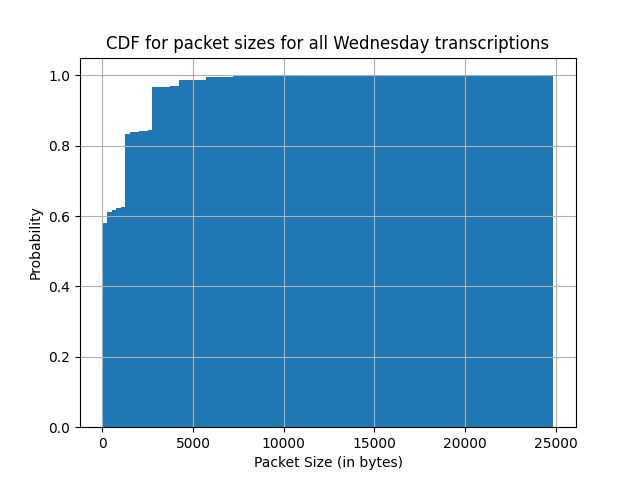
\includegraphics[width=0.85\textwidth]{final-report/img/packet-sizes_cdf.png}
    \caption{CDF for packet sizes}
    \label{fig-cdf-packet-sizes}
\end{figure}
%-------------------------------------------------------



%-------------------------------------------------------
\subsection{Schema}\label{sec-schema}
% descrieb the schema definition. Describe what characters we use, describe how we distinguish between the flow directions, describe the binning
The output of our data processing pipeline is a tsv file with four columns -- Source IP, Destination IP, Attack, Transcription. The IP addresses represent the communication endpoints. The Attack attribute contains a binary information whether the network flow is a attack or not. The Transcription attribute contains the transcription itself.

The transcription is a string of characters describing a network flow. We use 93 characters to describe flows by transcriptions. These are printable ASCII characters in the range from the exclamation mark character (\textit{!}) up to the tilde character (\textit{$\sim$}) where each character represents a captured packet size. Each character represents different packet sizes. The characters are ordered in the same chronological order as the packet captures.

The very first character, exclamation mark, is used to represent a silence in a communication. One such character represents a silence of 1 second. The 46 characters starting from the quotation mark included up to the \textit{O} character included are used to describe one direction of a communication. The 46 characters starting from the \textit{P} character included up to the tilde character included are used to describe the other direction of a communication.

Based on the research in the section \ref{sec-dataset-exploration} we utilized the characters in such way that the characters represent different bins of packet size. We reasonably chose binning based on the analysis of the figure \ref{fig-cdf-packet-sizes}. We encoded the packets of length $<= 2^{14}$ with first 30 characters, the packets of length $(2^{14}; 2^{16}]$ with the next 15 characters and the packets of length $> 2^{16}$ with the last (46th) character. Naturally, each communication direction utilizes its own character set as described in the section \ref{sec-dataset-exploration}. In every category the bins are of the same size. Meaning, in the first category there are 30 bins of the same size, in the second category there are 15 bins of the same size and in the last category there is just one bin.

%-------------------------------------------------------

\subsection{Output Data Set}

The output data set built from pcap files is a TSV file. The basic file structure is \textit{srcIP, dstIP, transcription}. The advanced file structure which contains also labels for network flows contains \textit{label} and \textit{attack} alongside the 3 mentioned attributes. An end-user will receive file of the basic structure if no file containing labels is specified. If such file is specified, the program tries to look up a label for each flow and assign a label and a type of attack to each entry of the output data set.

%-------------------------------------------------------


\subsection{Implementation}
% describe the software itself, the scripts for data processing, what language I used

\subsubsection{Data Processing Pipeline}
The software for processing the \textit{pcap} files and converting network flows into sentence-like transcriptions is a data processing pipeline consisted of two steps. The two-step process consists of extracting the necessary features from a \textit{pcap} file with go-flows and the 2nd step is the transcriptions building process itself based on the output from the 1st step. The data processing pipeline itself is a shell script that orchestrates the steps to be done in order to achieve the final output. The shell pipeline is located in \verb|/transcription/pipeline.sh|.


\subsubsection{Transcriptions Maker}
As mentioned above, the 2nd step of the data processing pipeline is the transcriptions building process. This is the core software of this project implemented in Python expecting a CSV file of a certain structure as an input and producing a TSV file containing the sentence-like transcriptions as the output. Let's call this software the transcription maker.

The input CSV file for this core software is an output produced from go-flows. The configuration file used for go-flows is located in \verb|/transcription/feature_extraction/pcap2pkts.json|. This configuration file makes go-flows produce a CSV file of the following header structure: \textit{flowStartMilliseconds, protocolIdentifier, sourceIPAddress, destinationIPAddress, ipTotalLength}. Since we are dealing with packets, the \textit{flowStartMilliseconds} attribute represents a timestamp of a packet. The \textit{ipTotalLength} attribute represents a size of a IP packet itself. The other attributes are self-explaining.

Transcription maker filters the TCP packets from the input CSV file and subsequently the TCP packets get ASCII characters assigned to them based on the \textit{ipTotalLength} attribute as described in the section \ref{sec-schema}. Then, the sentence-like transcriptions of all the flows are built and outputted.

The final structure of the output TSV file is the following: \textit{srcIP, dstIP, transcription}. If a file with labels assigned to the network flows was specified, the output TSV file additionally contains 2 more columns: \textit{label, attack}. Label is a binary label indicating whether a flow is attack or not. The attack attribute describes what type of attack it is.


\subsection{Testing}
For the testing purposes I decided to train Random Forest on top of bag of words. The goal was to achieve the highest possible accuracy for the \textit{attack} class as well as for the \textit{non-attack} class. Achieving overall accuracy on top of the whole test set is meaningless for us as our data set is imbalanced and therefore overall accuracy may distort results.

We used a very simple bag of words technique. For each entry of the data set (a transcription) we counted number of each word in a particular transcription. Basically, we transformed our data set of transcriptions to the data set where our dimensions represented the word counts in transcriptions. For better understanding, see an example at figure \ref{fig-bag-of-words-example}.

\begin{figure}[h!]
\centering
\begin{tabular}{ |c|c|c|c| }
 \hline
 srcIP & dstIP & attack & transcription \\
 \hline
 1.1.1.1 & 2.2.2.2 & 1 & AAp!D!p \\
 2.2.2.2 & 3.3.3.3 & 0 & P!PD \\
 \hline
\end{tabular}

\vspace{0.3cm}

\begin{tabular}{ |c|c|c|c|c|c|c| }
 \hline
 srcIP & dstIP & A & D & P & p & ! \\
 \hline
 1.1.1.1 & 2.2.2.2 & 2 & 1 & 0 & 2 & 1 \\
 2.2.2.2 & 3.3.3.3 & 0 & 1 & 2 & 0 & 1 \\
 \hline
\end{tabular}
\caption{Data set of transcriptions (on top) and bag of words data set (bottom)}
\label{fig-bag-of-words-example}
\end{figure}

We trained a Random Forest model on top of the bag of words data set. As our data set was imbalanced -- approximately 10:2 ratio of non-attacks to attacks -- we considered this during the Random Forest model training. To put a higher to attacks so that we simulate the balance of the classes.

% describe the results that I got (the confusion matrix, accuracy etc). Next describe how I constructed the train and test data set, how many entries the train and test data set contain



\section{Conclusions}




\bibliographystyle{plain}
\bibliography{references}


% \bibliographystyle{plain}

% \begin{thebibliography}{}

% \bibitem{cic-ids-dataset} Iman Sharafaldin, Arash Habibi Lashkari, and Ali A. Ghorbani, “Toward Generating a New Intrusion Detection Dataset and Intrusion Traffic Characterization”, 4th International Conference on Information Systems Security and Privacy (ICISSP), Portugal, January 2018


% % \bibitem{tshark-documentation} Wireshark.org. 2020. \textit{Tshark - The Wireshark Network Analyzer 3.4.0}. [online] Available at: \url{https://www.wireshark.org/docs/man-pages/tshark.html} [Accessed 28 November 2020].

% % \bibitem{python-popularity} Piatetsky, G., 2020. \textit{Python Leads The 11 Top Data Science, Machine Learning Platforms: Trends And Analysis - Kdnuggets}. [online] KDnuggets. Available at: \url{https://www.kdnuggets.com/2019/05/poll-top-data-science-machine-learning-platforms.html} [Accessed 28 November 2020].


% \end{thebibliography}

\end{document}
